\chapter{Основная часть}

\section{Определение структуры и состава основных фондов}

К активной части ОФ относятся те группы ОФ, которые непосредственно участвуют в процессе превращения предметов труда в готовую продукцию. Это передаточные устройства, силовые машины и оборудование, рабочие машины и оборудование, измерительные и регулирующие устройства и приборы.

\begin{table}[H]
	\caption{Активная часть ОФ}
	\label{tbl:active_struct}
	\centering
	
	\begin{tabular}{|l|c|}
		\hline
		Группа ОПФ & ФО \\ \hline
		Передаточные устройства & 1830 \\ \hline
		Силовые машины и оборудование & 1326 \\ \hline
		Рабочие  машины и оборудование & 29420 \\ \hline
		Измерительные и регулирующие устройства и приборы & 2485  \\ \hline
		Вычислительная техника & 2216 \\ \hline
		Всего & 37277 \\ \hline
	\end{tabular}
\end{table}

\begin{table}[H]
	\caption{Пассивная часть ОФ}
	\label{tbl:passive_struct}
	\centering
	
	\begin{tabular}{|l|c|}
		\hline
		Группа ОПФ & ФО \\ \hline
		Здания & 28642 \\ \hline
		Сооружения & 1765 \\ \hline
		Транспортные средства & 29420 \\ \hline
		Инструмент & 2485  \\ \hline
		Производственный и хозяйств. инвентарь и принадлежности & 276 \\ \hline
		Всего & 62588 \\ \hline
	\end{tabular}
\end{table}

\begin{figure}[H]
	\centering
	\caption{Соотношение активной и пассивной части ОФ}
	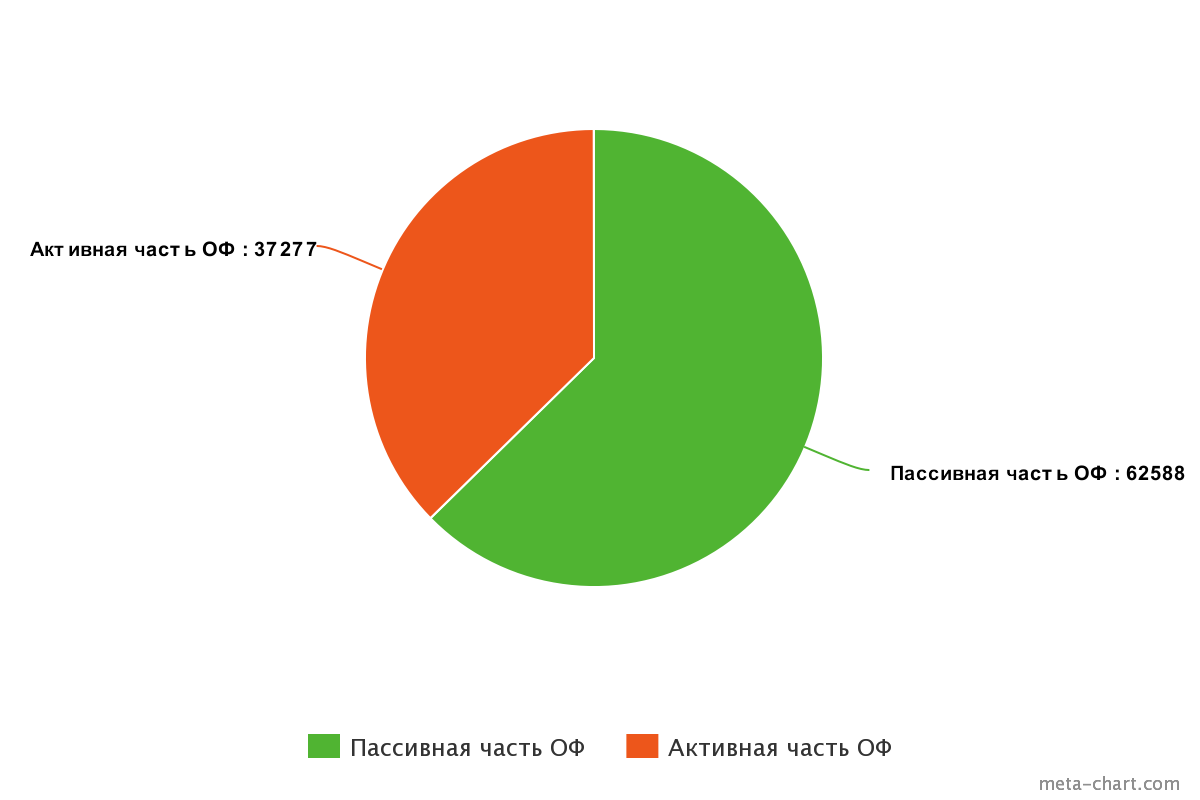
\includegraphics[width=\textwidth]{images/a_p_chart.png}
\end{figure}

\begin{table}[H]
	\caption{Удельный вес отдельных групп ОФ в общей их стоимости}
	\centering
	
	\begin{tabular}{|p{10cm}|c|}
		\hline
		Группа ОПФ & Удельный вес, \% \\ \hline
		Здания & 40,80696405 \\ \hline
		Сооружения & 2,514639046 \\ \hline
		Передаточные устройства & 2,60724615 \\ \hline
		Силовые машины и оборудование & 1,889184915 \\ \hline
		Рабочие  машины и оборудование & 41,91539985 \\ \hline
		Измерительные и регулирующие приборы и устройства, лабораторн. обор-е & 3,54044081 \\ \hline
		Вычислительная техника & 3,157189873 \\ \hline
		Транспортные средства & 2,199774894 \\ \hline
		Инструмент & 0,9759364 \\ \hline
		Производственный и хозяйств. инвентарь и принадлежности & 0,393224009 \\ \hline
	\end{tabular}
\end{table}

\begin{figure}[H]
	\centering
	\caption{Удельный вес отдельных групп ОФ в общей их стоимости}
	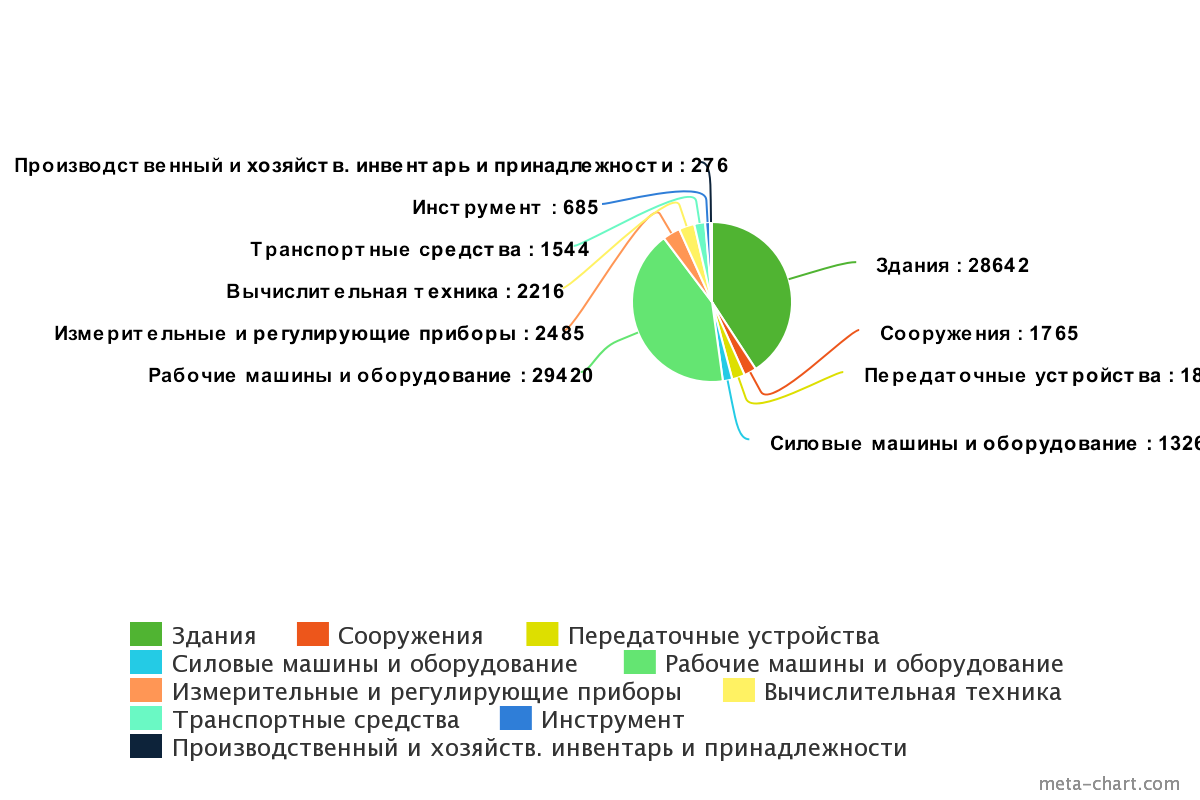
\includegraphics[width=\textwidth]{images/udel_ves_grup.png}
\end{figure}


\begin{table}[H]
	\caption{Возрастная структура}
	\centering
	\begin{tabular}{|m{7cm}|c|c|}
		\hline
		Группа ОПФ & Средний фактический срок службы & ФО\\ \hline
		\multicolumn{3}{|c|}{До 5 лет} \\ \hline
		Измерительные и регулирующие приборы и устройства, лабораторн. обор-е & 4.5 & 2485 \\ \hline
		Вычислительная техника & 3 & 2216 \\ \hline
		Инструмент & 3 & 685\\ \hline
		\multicolumn{3}{|c|}{От 5 до 10 лет} \\ \hline
		Рабочие  машины и оборудование & 8 & 29420 \\ \hline
		Транспортные средства & 5 & 1544\\ \hline
		Производственный и хозяйств. инвентарь и принадлежности & 6 & 276\\ \hline
		\multicolumn{3}{|c|}{От 10 лет} \\ \hline
		Здания & 35 & 28642 \\ \hline
		Сооружения & 15 & 1765\\ \hline
		Передаточные устройства & 12 & 1830\\ \hline
		Силовые машины и оборудование & 16 & 1326 \\ \hline
		
	\end{tabular}
\end{table}

\begin{table}[H]
	\caption{Удельный вес отдельных возрастных групп в общей стоимости ОФ}
	\centering
	\begin{tabular}{|c|c|}
		\hline
		Возрастная группа & Удельный вес \\ \hline
		До 5 лет & 0,07673567083 \\ \hline
		От 5 до 10 лет & 0,4450839875 \\ \hline
		От 10 лет & 0,4781803416 \\ \hline

	\end{tabular}
	
\end{table}

\section{Оценка основных фондов}




\section{Расчет амортизации основных фондов}

\section{Расчет показателей использования основных фондов}